\thispagestyle{plain}
\chapter{Background}

Before we can look at the approach that we used to answer the research questions, we need to cover some essential information. First, we look at the definition of partitions and how indexes partition data using partitioning functions in Section \ref{bg:partitions}. After that, we cover hybrid indexes and their structure in Section \ref{bg:hybrid}, where we also lay the foundation for the index that we used later on. To understand the idea behind an algorithm that will be used, we look at numerical differentiation to approximate the derivative of a function in section \ref{bg:numerical}.

\section{Partitions and Partitioning functions}\label{bg:partitions}
Let us first look at the definition of a partition in the rigorous mathematical sense to transfer this to the field of index structures. The following definition is taken from \citeauthor{Lucas1990} \cite{Lucas1990}.

\vspace{0.5cm}
\noindent \textbf{Definition 3.1 (Partition):}

\noindent Let $M \neq \emptyset$ be a nonempty set. A partition $P$ of $M$ is a collection of subsets of $M$ with the following properties:

\begin{enumerate}
    \item[P.1] $\forall p \in P: p \neq \emptyset$
    \item[P.2] $\forall p,q \in P: p \neq q \implies p \cap q = \emptyset$
    \item[P.3] $\bigcup_{p \in P} p = M$
\end{enumerate}

\noindent To summarize, a partition $P$ of $M$ is a collection of nonempty (P.1), mutually disjoint (P.2) subsets of $M$, whose union exhausts all of $M$ (P.3).

\vspace{0.5cm}
To adapt this to data partitioning for index construction, we can look at the keys $K = \{k_1, k_2, ..., k_n\}$ over which we want to construct our index. If we look at typical B$^+$-trees, the data partitioning is induced by the contents of the leaf nodes. B$^+$-trees don't allow empty nodes (P.1), there is only one possible way to traverse through the index given a certain key, which means that the leaf nodes' contents are disjoint (P.2) and if the index was built over the whole key space $K$, every key will be present in some leaf node (P.3). 

To formalize the partitioning inside a (logical) index, we need to look at the (logical) nodes separately. According to \citeauthor{Dittrich2021} \cite{Dittrich2021}, one can define a logical node as follows:

\vspace{0.5cm}
\noindent \textbf{Definition 3.2 (Logical Node):}
A logical node is a tuple (p, RI, DT):
\begin{enumerate}
    \item $p: [R] \rightarrow D$ is a \textbf{partitioning function} on the relational schema $[R] : \{ [A_1 : D_1, ..., A_n : D_n] \}$. $p$ may be undefined.
    \item $RI : D \rightarrow \mathcal{P}(N)$ is the \textbf{routing information}, where $N$ is a set of nodes and $\mathcal{P}(N)$ is the power set of $N$. Each element of $D$ (target domain of $p$) is mapped to a subset of nodes in $N$. $RI$ may be undefined.
    \item $DT$ is the \textbf{data}. It is a set of tuples with relational schema $[R]$. $DT$ may be empty.
\end{enumerate}

\noindent Using this definition, we can see how a partitioning functions interacts with the routing information to organize an index. When we look at the example from above, we can see that the partitioning inside a B$^+$-tree happens through the partitioning function $p(t) = t.key$ and the routing information maps certain ranges (that are created in the B$^+$-tree through the keys in inner nodes) to the corresponding child nodes.

//TODO: grafik aus GENE papier

//TODO: noch ein Beispiel??

\section{Hybrid Index Structures}\label{bg:hybrid}
To understand the motivation of this work and the general structure of the index that will later be used in the evaluation of partitioning algorithms, we will now look at the framework presented by \citeauthor{Dittrich2021} \cite{Dittrich2021} in more detail.

We have already seen logical nodes in definition 3.2, which introduced the concept of partitioning function and routing information to construct an index. Although we have use the B$^+$-tree as an example above, we need to note that the routing information is more general than just a tree-like structure. In theory, there is no restriction to the layout of the graph that is created by the routing information. Additionally, this framework is purely logical yet, i.e.~no physical layout is assumed. As long as all the nodes in the target domain of $RI$ are part of the graph, we call this graph \textbf{Complete Logical Index}. The power of this indexing framework lies in its generalisation of common index structures. As we have seen, we can represent B$^+$-trees, Radix Trees and Learned indexes trough this framework in the form of logical nodes. And as a complete logical index is just a graph of logical nodes, we easily can connect different node types to form a \textbf{Hybrid Logical Index}. 

In the next step to realize this framework, we have to move from the purely logical index to a physical index by specifying how the logical node with its routing information and data should be physically represented. The first part to this specialization is to determine the search method that should be used in the RI and DT parts of the node to find key/value pairs. Presented options include linear search, binary search, interpolation search, exponential search, chained hashing and linear regression. Note that the choice here can already have an impact on the data layout that should be used inside the node, e.g.~for binary search, we naturally require a sorted layout. Other options for the data layout include column vs row layout, whether to use a compression and which one or any other suitable hybrid data layout.

With this multitude of options to create a physical index, we need to decide which configuration we should use for a specific use case. This is done using a genetic breeding algorithm. It starts with an initial population of physical index structures and performs a set amount of iterations in the genetic search. This includes sampling from the current population and determining the fittest index together with the median fitness across the sample. After that, several mutations are randomly drawn for this fittest index and applied. If this new mutated index has a better fitness than the median fitness from before it is added to the population (replacing the worst index there if needed) and the whole process is repeated. After the set amount of iterations, the fittest index in the population is selected. The possible mutations are drawn from a distribution that allows to prioritize certain mutations over others. Mutations include changing the data layout or the search method of the RI or DT part, merging sibling nodes horizontally/vertically or splitting nodes horizontally/vertically. Note that the selection of the fittest index is completely dependent on the selected performance measure and the fitness functions representing it. A possible goal of the genetic optimization could be the runtime of the index on a given workload, where the fitness function could just be the median runtime of the workload over a given number of runs. Other goals include memory or energy-efficiency.

As the amount of iterations is set as a global parameter, the starting population plays a big role in how good a genetically bred index can become. If we would already start with a reasonable population, chances are higher that a good index can be found in the set amount of iterations. The authors present four possible ways to determine the initial population:

\begin{enumerate}
    \item We start with a single physical node that does not contain data yet.
    \item We start with a single physical node that contains all the data with a random or manually set data layout and search method.
    \item We use bottom-up bulkloading where data layout and search method are picked randomly. The logical index structure is very similar to a B$^+$-tree in this case.
    \item We start with a index that represents a state-of-the-art hand-crafted index. The genetic algorithm here serves mainly for fine-tuning this already established index.
\end{enumerate}
\noindent Note that these starting options do not incorporate the workload information that will be used to find the fittest index in the population. However, if we were to already use that information in the starting population, we could be able to find a better starting point for the genetic search than the described options above. This is a main motivation behind my work: using the workload information to find a partitioning that can be used for the bulkloading of an index similar to point 3) above. It would be still fairly general and allow the genetic search a good amount of modifications, while setting physical design options optimized for the workload already in the beginning.

\begin{itemize}
    \item Advantages: optimize for subproblems, combine to one index
    \item challenges: correct combination of these structures (e.g.~routing through data structure)
\end{itemize}


\section{Numerical Differentiation}\label{bg:numerical}
//TODO: visulize disadvantage: periodic function

In the coming sections, we will discuss an algorithm that aims to find the boundaries of a plateau of a function. As we will not work on a continuous function, but a discrete one, we need to look at a way that enables us to approximate the derivative of a discrete function. This will be useful, as a plateau is identified by a vanishing derivative.

To calculate the derivative of a function $f$ at a point $x$, we know we have to evaluate the limit 
$$
\lim_{h \rightarrow 0} \frac{f(x+h) - f(x)}{h}
$$

However, we cannot evaluate this limit if we only have a discrete function. For this purpose, we can use finite differences to approximate the derivative. There are three common ways for this kind of approximation:
\begin{enumerate}
    \item Forward difference approximation: $\frac{f(x + h) - f(x)}{h}$
    \item Backward difference approximation: $\frac{f(x) - f(x-h)}{h}$
    \item Central difference approximation: $\frac{f(x + \frac{h}{2}) - f(x - \frac{h}{2})}{h}$
\end{enumerate}

\begin{figure}
    \centering
    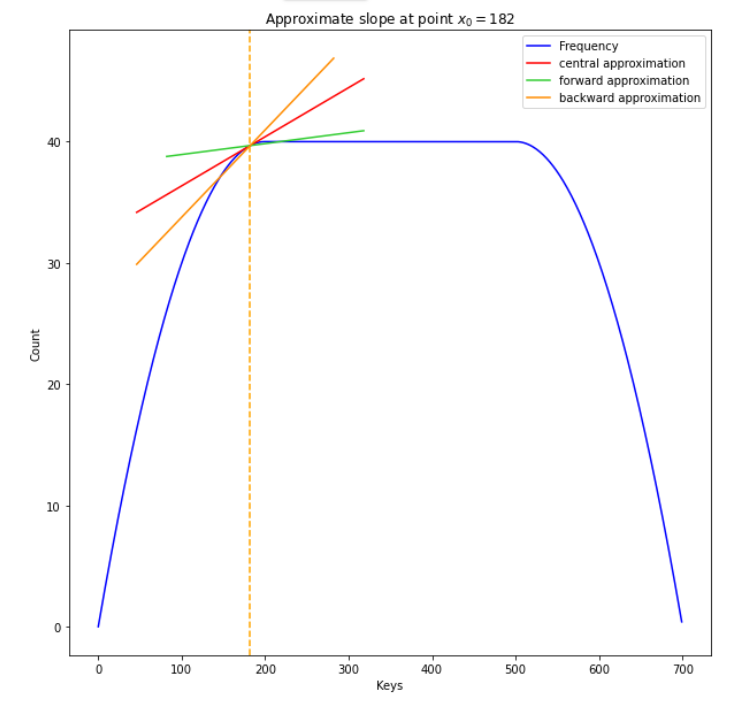
\includegraphics[width=0.6\textwidth]{figures/approx_1.png}
    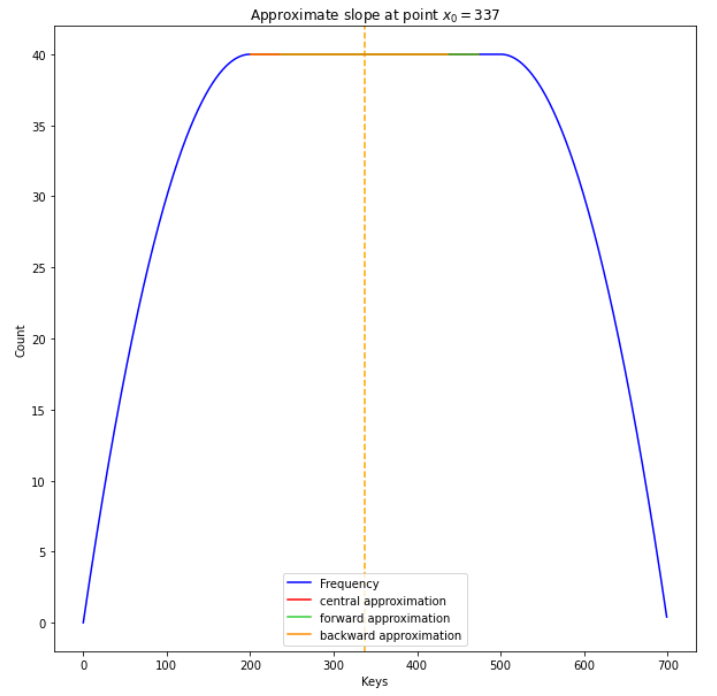
\includegraphics[width=0.6\textwidth]{figures/approx_2.png}
    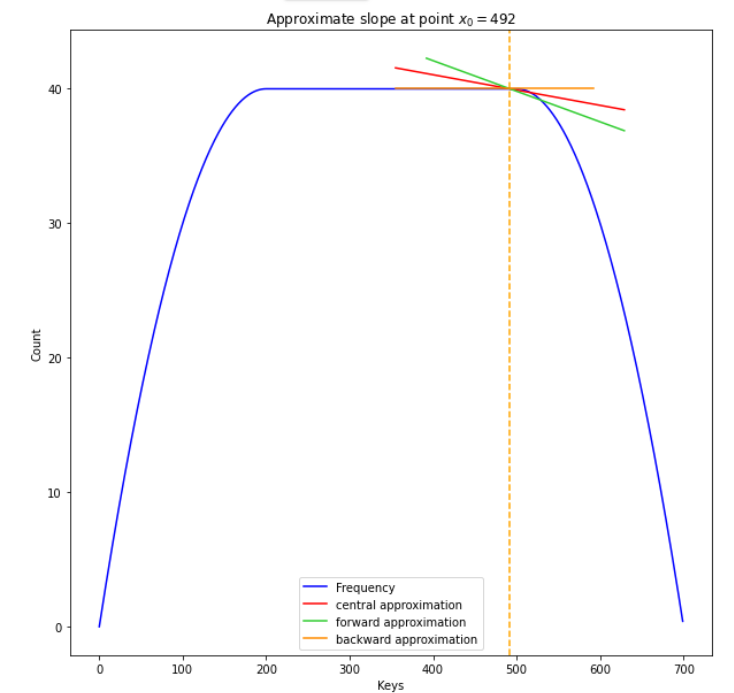
\includegraphics[width=0.6\textwidth]{figures/approx_3.png}
    \caption{Comparison of the difference approximations}
    \label{fig:approximations}
\end{figure}

To motivate the later use of the approximations for identifying plateaus, we can look at Figure \ref{fig:approximations}. All images show the three difference approximations at different points, where they are used to approximate the slope of the blue function. In the first image, we can see that we are at the start of the plateau, but only the slope of the forward approximation is nearly zero, the other two are still quite different to zero. This is why we can use the forward approximation to find the start of a plateau. On the second image, we see that when we are inside the plateau, all approximations are zero, so we would choose the central approximation as it is more robust to outliers in one single directions. And in the last image, we see the approximations still quite a bit before the end of the plateau, and we can recognize that only the backward approximation is still near zero. If we would use one of the others to find the end of a plateau, we had already stopped before the actual end is reached.

As these are only approximations, they are not exact representations of the actual derivative and produce an error. Using Taylor's expansion, we can show that for the central difference approximation, this error is in $O(h^2)$ while it is in $O(h)$ for the forward and backward difference approximations. The central difference approximation is, therefore, more accurate but has the downside that it can yield zero estimations for periodic functions.

